In this section, I develop methods to attribute mass comments to the campaigns that mobilized them and measure the intensity of preferences expressed. 
To link individual comments to the more sophisticated lobbying efforts they support, I use text reuse and topic models to identify clusters of similar comments, reflecting formal and informal coalitions. Comments with identical text (if any) indicate which groups and coalitions ran a mass comment campaign. Within each campaign, I measure the intensity and potential for the movement to grow. To measure intensity, I examine the ratio of high-effort and low-effort comments. To measure potential to grow, I measure the number of comments mobilized indirectly by the campaign (i.e. those that support a campaign but do not include text provided by the campaign).
The result is several new measures that paint a picture of mass commenting. 
% TO DO 
% Using these new measures of public engagement in agency rulemaking, I identify the conditions under which it occurs and produces different politically-relevant information. 

\subsubsection{Who lobbies?}
Previous studies of rulemaking stress the importance of coalitions \citep{Yackee2006JOP}. Scholars have measured coalitions of organized groups but have yet to be able to attribute citizen comments to the coalition that mobilized them.
% Metadata on participants in rulemaking including the date and author of comments (often including the type of author, i.e. business, business group, citizen, public interest group, etc.)% and briefs
% allows me to track and compare relative alignment across venues and over time to assess whose ideas and interests are reflected at each stage of policymaking and in policy processes over time. % and review, for example from a statute or executive order, to the agency rule(s), to review by the White House, to court opinions. 


\paragraph{Data.} I collected a corpus of approximately 70 million comments on over 300,000 proposed rules via the regulations.gov API. I then linked these comments to other data on the rules from the Unified Agenda and Office of Information and Regulatory Affairs Reports on draft rules sent to them for review. See the Appendix for summary statistics for these data.

Unfortunately, metadata on the authors of comments and their organizational affiliations are inconsistent and incomplete. As this information is key to identifying influential actors, improving these data was a significant data-organization task. 
First, I identified organizations responsible for mobilizing 100 or more comments with repeated text, either identical text or partially unique texts that contain shared language.\footnote{Specifically, I identify comments that are not identical but share a 10-word (or ``10-gram'') string using a moving window function looping over each possible pair of texts to identify matches. For more about this method and comparison to related partial matching methods such as the Smith-Waterman algorithm, see \citet{Casas2017} and \citet{Judge-Lord2017}}.
I then searched comment texts for mentions of these organizations' names to complete missing information on the mobilizing organization.
% Further text matching of organization and individual names across texts, especially those named as comment authors will help systematically link individuals to the groups that mobilized them. % who may participate in different coalitions and under different names over time. 
% This helps to identify formal coalitions of organizations that sign onto the same comment as well as experts and citizens mobilized by advocacy campaigns to submit separate comments.
 The top 100 mobilizing organizations mobilized between 55 thousand and 4.2 million comments. Figure \ref{fig:toporgs} shows the top organizers of comments posted to regulations.gov.

\begin{figure}
    \centering
        \caption{Top mobilizers of comments posted to regulations.gov}
    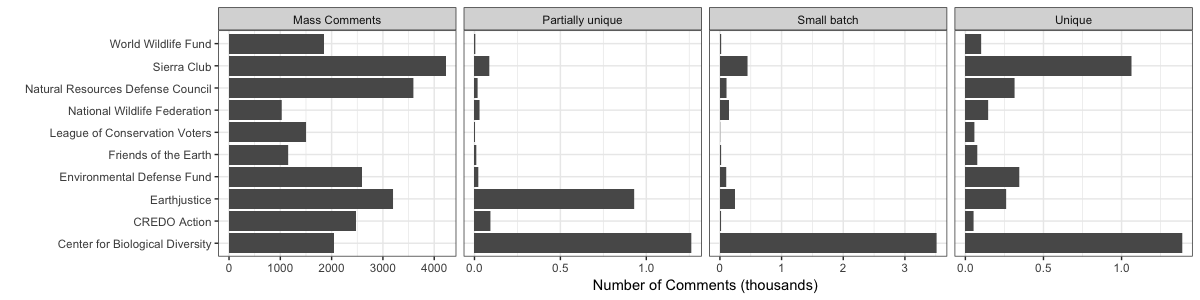
\includegraphics[width = 6.5in]{Figs/toporgs.png}
    \label{fig:toporgs}
\end{figure}

Having identified who is participating in rulemaking, the next step is to identify who is lobbying together.

\subsubsection{Who lobbies together?}
% political information example 
The Oceana coalition framed its mass mobilization effort to curb the  Bureau of Ocean Energy Management's 2017 Proposed Offshore Oil and Gas Leasing Program as a ``petition signed by 67,275 self-proclaimed United States residents,'' suggesting that organizations consider these efforts as akin to petitions. In the same statement, Oceana also claimed the support of ``more than 110 East Coast municipalities, 100 Members of Congress, 750 state and local elected officials, and 1,100 business interests, all of whom oppose offshore drilling,'' suggesting that claims of public and elected official support aim to provide similar kinds of political information. 

% lobbying together - cosigning 
When actors sign onto the same comment, it is clear that they are lobbying together. %This generally takes two forms. Businesses and groups representing allied industries often co-sign carefully-crafted technical suggestions that reflect their common interest. %This is likely to occur when the benefits of coordination outweigh the costs \citep{Yackee2006JOP}. 
% The other form this take is public campaigns that ask citizens to submit a form letter.%, often alongside other actions such as protests. 
%These occasional bursts of civic participation may affect rulemaking \citep{Coglianese2001}, but this is yet to be tested. 
%In the first form, many of the businesses are repeat players and I record them individually. In the second form, the advocacy groups are repeat players, and I recorded their participation, but it would be citizens who participate are likely not and I record the number of these comments as an amplitude parameter for the text they signed and I attribute form-letter texts to the group backing the campaign that mobilized them.
% TO DO - TOPIC MODELING APPROACH
However, various businesses, advocacy groups, and citizens often comment separately even when they aligned. The comment process is open to anyone and it is often not worthwhile for all actors to coordinate their messages. 
Thus, in addition to mapping text re-use, I adapt several statistical models (k-means clustering and Bayesian classifiers) of text to classify comments into coalitions. % Classifying comments into common groups is a task well suited for a single-member topic model.% \footnote{
% This is in contrast to the mixture model I use to estimate the distribution of multiple topics in each document and each coalition in section \ref{principals-methods}
% }
I cluster documents by the frequency with which they use different words. Being classified together does not mean that the documents all address exactly the same distribution of substantive issues, just that they use similar words relative to the full set of documents.
I start by modeling all comments on each rule (collapsing identical comments to one document) with two and three topics, which I will then inspect to see how well the comments of named organizations were classified. If the two topic model most sensibly describes the conflict, I label these clusters ``pro'' and ``con'.' If the three-topic model more sensibly describes the conflict, I label these clusters as ``pro, con, other.'' If neither fits well, I increase the number of clusters as needed. I repeat this process for each of the several 




% TODO TESTING CAUSAL SEGMENT 
% In terms of the causal process theorized above, this section focuses on measuring and explaining organizations' lobbying choices (i.e. to only provide technical information or to also mobilize) and public response to mobilization campaigns (the frequency and effort with which people engage). The key explanatory variable is public support for the campaign. The bold arrows in figure \ref{fig:causal-whymail-test} indicate the relationships of interest for this step.

% \begin{figure}[h!]
    \centering
    \caption{Step 1: Explaining Mass Mobilization and Mass Engagement} 
    \label{fig:causal-whymail-test}
\tiny
\begin{tikzpicture}[%
    node distance=1.2cm,
    auto,
    text width=1.5cm,
dnode/.style={diamond, align=center, aspect=2, fill=green!5,draw=green!60, very thick, minimum size=2cm},
squarednode/.style={rectangle, align=center, aspect=1, draw=red!60, fill=red!5, thick, minimum size=1cm},
pnode/.style={ellipse, align=center, aspect=1, draw=black!60, fill=black!5, thick, minimum size=1cm},
title/.style={rectangle, align=center, aspect=1, minimum size=2cm},
]

% Group Nodes
\node[pnode]      (groupdemands) {Group Demands};
\node[dnode]        (groupdecides) [right=of groupdemands] {Lobbying Strategy};
\node[squarednode]      (groupinfo) [right=of groupdecides] {Technical Information};


% Group Lines
\draw[->] (groupdemands.east) -- (groupdecides.west);
\draw[->] (groupdecides.east) -- (groupinfo.west);

% Titles
% \node[title]      (1) [above=of draft] {Policy};
% \node[title]      (2) [above=of groupdemands] {Preferences};
% \node[title]      (4) [above=of groupinfo] {Information/ Signal};
% \node[title]      (3) [above=of groupdecides] {Observed Behavior};
% \node[title]      (5) [above=of policy] {Policy'};

\node[text centered]      (mobilizing) [below=of groupdecides] {Mass\\ Mobilization};

% political info
\node[rectangle, minimum width =2cm, minimum height = 3cm, draw=red!60, fill=red!5,  thick]      (politicalinfo) [below=of groupinfo] {};

\node[text centered]      (politicalinfotext) [below=of groupinfo] {Political Information};

\node[text centered]      (mobilizing) [below=of groupdecides] {Mass\\ Mobilization};

\node[squarednode]      (publicinfo) [below=of politicalinfotext] {Perceived Public Opinion};
\node[dnode]      (publicdecides) [left=of publicinfo] {Mass\\ Engagement};
\node[pnode]        (publicdemands) [left=of publicdecides] {Latent Public Demands};


% public Lines
\draw[->, line width=2] (publicdemands.east) -- (publicdecides.west);
\draw[->, line width=2] (publicdemands.north east) -- (groupdecides.south west);
\draw[-, line width=2] (groupdecides.south) -- (mobilizing.north);
\draw[->, line width=2] (mobilizing.south) -- (publicdecides.north);
\draw[->] (publicdecides.east) -- (publicinfo.west);



\end{tikzpicture}
\end{figure}
\normalsize





% OUTCOMES OF A CAMPAIGN
\subsubsection{Measuring the volume, intensity, and potential contagion of public engagement.}

%\textbf{Level of engagement.} 
% Dependent variables include the number of people engaged and the effort per comment.
%I argue that activists' opportunities and strategies explain variation in engagement, which I measure in several ways. 
I measure variation in engagement in several ways. 

\paragraph{Volume.} 
First, I measure the total number of comments on the rule. As commenting are the results of two processes: deciding to lobby at all and then deciding to mobilize, the distribution contains many cases where groups may have had success mobilizing but never reached the choice of whether to mobilize or not. Perhaps they were unaware of the draft rule. Once the decision to mobilize has been reached and made, the result of mobilizing is a count process. Thus, I expect the count of comments to follow a zero-inflated negative binomial distribution. When focusing on coalitions, we have already subset to cases where mobilization occurred and thus commenting can now be considered a regular count process. 

\textbf{Effort.} I measure effort per comment by the number of words people write, omitting any to text longer than 10 words that is not unique, usually because it was provided by a mobilizing organization. % effort example 
For example, using the form shown in \ref{fig:sierra}, the Sierra Club mobilized more than 47,710 people to submit exactly the same text on the delay of the methane pollution rule, but 7,452 people also took the time to write a personalized comment in addition to the text provided. However, we may not observe people who have low levels of passion for the issue because they either do not cross the effort threshold required to comment or opt to write nothing more than the form letter. I consider the low end of the distribution of words to be truncated.

% contagion
\textbf{Contagion.} Mass-comment campaigns have wildly different results. Some gather a clean 10,000 copies of (signatures on) the same comment and call their work done. Others ``go viral''---inspiring a mess of further engagement where the original messages are translated through social media posts and news stories.
To identify people who were plausibly mobilized indirectly by a campaign, I count the number of people who use similar distribution of words to that of the form letter but fewer than 10 words matching any other comment. This is regular count process.

% \begin{quote}
% \textbf{Dependent Variables:} 

% Model 1) Total comments $\sim$ zero-inflated negative binomial; 

% Model 2) Comments per coalition $\sim$ negative binomial; 

% Model 3) Effort per comment $\sim$ truncated normal; 

% Model 4) Contagion $\sim$ negative binomial. 

% % Model 4) Type of campaign $\sim$ multinomial. 
% \end{quote}

% The dependent 2-4 are built using text reuse and bayesian classifiers\footnote{
% Ultimately something similar to the correlated topic model \citep{Blei2005}, possibly with lexical priors \citep{Fong2016} based on organizational comments
% },
% one observation per coalition per rule. Explanatory variables include agency alignment with Congress and the president (models 1-4), coalition unity and alignment (models 2-4), and coding coalitions as driven more by public or private interests (models 2-3).%, part of the DV in model 4).










